\section{Image Processing}

\begin{figure}
\centering
  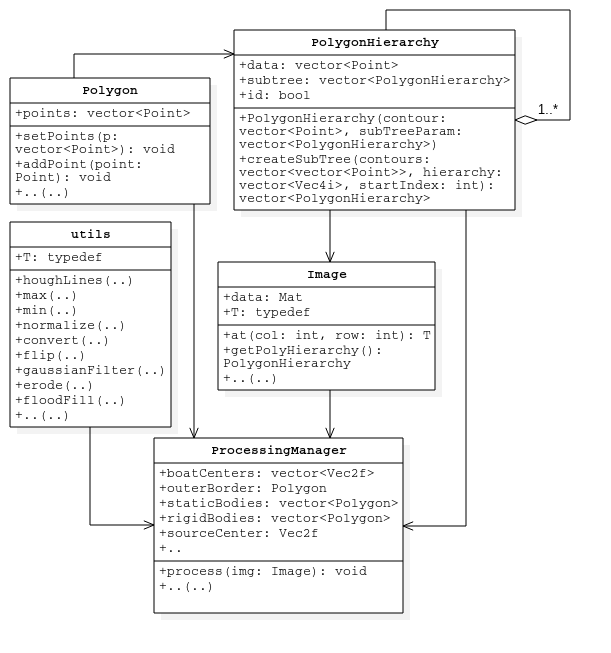
\includegraphics[scale=0.6]{img/ImageProcessing/UML_ImgProc_PNG.png}
\caption{UML diagram for the image processing code\label{fig:UMLImgProc}}
\end{figure}

One of Grand Theft Boat's USPs is the freedom for players to fully customize their level maps. Players can design complex maps replete with shorelines, connected water bodies, and floating spherical obstacles of varying radii. All this can be done using a simple computer graphics software like Gimp (Linux), MS Paint (Windows) and Paintbrush (Mac). 

In order to extract information about the terrain and participating bodies, the team relied on processing the input image through extensive use of the OpenCV library. This chapter describes the workflow involved in this stage. The broad structure of the image processing code is shown in Figure \ref{fig:UMLImgProc}.

\subsection{Level Terrain Specification}

\begin{figure}
\centering
  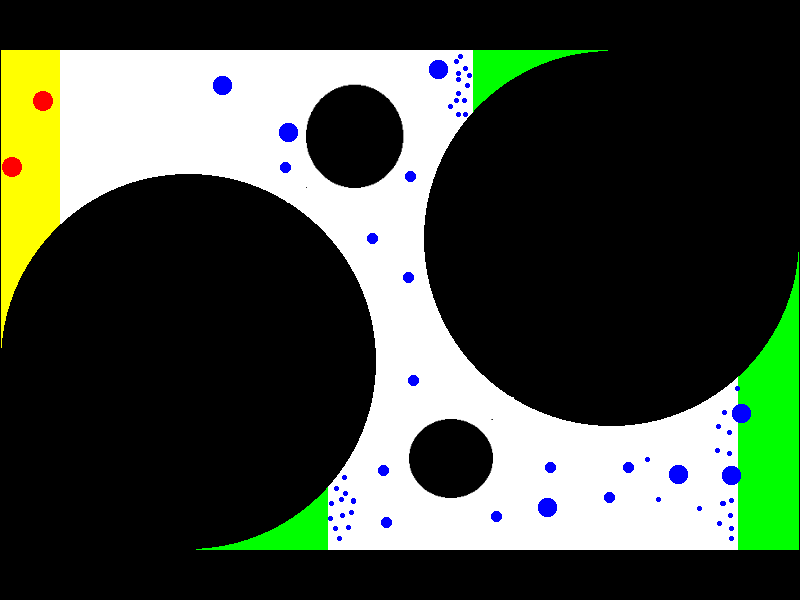
\includegraphics[scale=0.4]{img/ImageProcessing/LevelImages/img_0.png}
\caption{A typical player input for specifying the desired layout of the level\label{fig:LevelInput}}
\end{figure}

Figure \ref{fig:LevelInput} shows an example of a player's level specification.
\begin{itemize}
	\item Regions colored black represent land. This part of the domain is not a part of the solution field. The part of the black that borders the white region is treated as a rigid boundary.
	\item White-colored regions represent the water body. This space is the actual solution domain of the fluid.
	\item Green patches represent sources of momentum for the fluid.
	\item Yellow patches are sinks for the fluid. (See the section on LBM for the mathematical meaning of sources and sinks.
	\item Red spheres indicate the initial position of the player boats.
	\item Blue spheres create obstacles as rigid bodies.
\end{itemize}


\subsection{Pre-Processing}

Many a time, the image supplied by the player may need to be pre-processed for improving boundaries between terrain types. Once given as input to the \verb|ProcessingManager|, the input image undergoes the following sequence of filters:

\begin{enumerate}
	\item \textit{Flip image}: 
	
	\verb|img = img::flip(img, true, false);|
	
	Flipping the image along the y-axis is necessary because the coordinate system of a standard image has its origin on the top-left corner, while standard fluid codes begin indexing from the bottom-left corner.

	\item \textit{Gaussian filter and opening}

	\verb|blurred = img::gaussianFilter(img, 7, 2);|

	\verb|opened = img::opening(blurred, structuringElement, 2);|
	
	The gaussian filter and opening helps eliminates fuzzy borders of adjacent colors, making them sharper. See Figure \ref{LevelImages}(a).

	\item \textit{Thresholding}

	\verb|thresholded = applyThresholding(opened);|
	
	Thresholding applies yes-no filters on the image based on the colors of different domain types. This provides the \verb|ProcessingManager| with a boolean (black-white) image for each domain type, which is then used to extract domain information.

\end{enumerate}

